\documentclass[12pt]{article}
\usepackage[utf8]{inputenc}
\usepackage{amsmath, amssymb}
\usepackage{graphicx}
\usepackage{hyperref}
\usepackage{geometry}
\usepackage{algorithm}
\usepackage{algpseudocode}
\usepackage{amsmath}
\usepackage{mhchem}
\usepackage{booktabs}
\usepackage{subcaption}
\geometry{margin=1in}

\title{Hartree-Fock and MP2 Implementation Report}
\author{Arnav Brahmasandra, Jay Shen, Enoch Woldu}
\date{\today}

\begin{document}

\maketitle

\begin{abstract}
This report documents the implementation of the Hartree-Fock (HF) and Møller-Plesset perturbation theory (MP2) methods as developed in this repository. The focus is on the theoretical background, algorithmic details, and computational results obtained from the code.
\end{abstract}

\section{Introduction}
The Hartree-Fock method is a foundational approach in quantum chemistry for approximating the electronic structure of atoms and molecules. MP2 provides a post-Hartree-Fock correction to account for electron correlation effects. This report describes the implementation and results of these methods.

\section{Theoretical Background}
\subsection{Hartree-Fock Method}
The Hartree-Fock (HF) method approximates the many-electron wavefunction as a single Slater determinant of molecular orbitals, leading to a set of coupled integro-differential equations known as the HF equations. These equations are solved iteratively using the self-consistent field (SCF) procedure: starting from an initial guess for the orbitals, the Fock matrix is constructed, diagonalized to obtain new orbitals, and the process is repeated until convergence. Basis sets, typically composed of atomic orbitals or Gaussian functions, are used to represent the molecular orbitals and make the calculations tractable.

\subsection{MP2 Correction}
The Møller-Plesset perturbation theory of second order (MP2) provides a systematic way to include electron correlation effects that are neglected in the Hartree-Fock approximation. In MP2, the total electronic energy is corrected by adding a second-order perturbative term, which accounts for the interactions between electron pairs that are not captured by the mean-field HF approach. The MP2 energy correction is computed using the HF molecular orbitals and their corresponding energies, and involves summing over all possible double excitations from occupied to virtual orbitals. This correction typically lowers the total energy and yields more accurate results for molecular properties, especially in systems where electron correlation plays a significant role.

\section{Implementation Details}

\subsection{Code Structure}

The codebase is organized into modular components under the \texttt{src/} package. It includes \texttt{molecule.py} for representing molecular systems, and \texttt{integrals.py} for computing one- and two-electron integrals via PySCF. The Hartree-Fock SCF procedure is implemented in \texttt{scf.py}, and MP2 correlation energies are computed in \texttt{mp2.py}. \texttt{energies.py} handles the calculation of total energies including nuclear repulsion, while \texttt{orbital\_plot.py} enables 3D visualization of molecular orbitals using PyVista. The \texttt{utils.py} module contains utility functions needed for various tasks, and the \texttt{plot\_utils.py} module provides additional plotting functions. The \texttt{examples/} folder contains usage demos for common molecules, \texttt{tests/} includes unit tests and PySCF-based validation, and \texttt{main.py} provides a command-line interface to run full SCF/MP2 workflows and visualize selected orbitals.

\subsection{Algorithms}

\subsubsection*{Hartree-Fock Self-Consistent Field (SCF)}

We implemented a Hartree-Fock SCF procedure which iteratively solves the Roothaan equations:
\[
\mathbf{F} \mathbf{C} = \mathbf{S} \mathbf{C} \boldsymbol{\varepsilon}
\]
where $\mathbf{F}$ is the Fock matrix, $\mathbf{C}$ is the matrix of molecular orbitals, $\mathbf{S}$ is the overlap matrix, and $\boldsymbol{\varepsilon}$ is the diagonal matrix of orbital energies. The density matrix is updated at each iteration until convergence is achieved. Pseudocode for our SCF procedure and an orthogonalization solution to the Roothaan equations are provided in Algorithms \ref{alg:scf} and \ref{alg:roothaan}. 

\begin{algorithm}[H]
    \caption{Hartree-Fock Self-Consistent Field (SCF) Method}
    \begin{algorithmic}[1]
    
        \Statex \textbf{Input:} Atomic orbital basis set $\{\phi_i\}$; Convergence criteria $\epsilon$
        \Statex \textbf{Output:} Electronic energy $E_{el}$, MO energies $\boldsymbol{\varepsilon}$, MO coefficients $\mathbf{C}$, Density matrix $\mathbf{P}$
        
        \State $G_{ijkl} \gets (\phi_i\phi_j|\phi_k\phi_l)$ \Comment{AO exchange integral matrix from PySCF}
        \State $S_{ij} \gets \langle \phi_i | \phi_j \rangle$ \Comment{AO overlap matrix from PySCF}
        \State $T_{ij} \gets \langle \phi_i \: | \: -\frac{1}{2}\nabla^2 \: |\: \phi_j \rangle$ \Comment{AO kinetic energy matrix from PySCF}
        \State $V_{ij} \gets \langle \phi_i \: | \: -\sum_k^{\text{nuclei}} \frac{Z_k}{r_k} \: | \: \phi_j \rangle$ \Comment{AO nuclear potential energy matrix from PySCF}
        \State $H_{ij} \gets T_{ij} + V_{ij}$ \Comment{Core Hamiltonian matrix}
        \State $P_{ij} \gets 0$ \Comment{Density matrix}
        
        \While{$\Delta E_{el} > \epsilon$}
            \State $F_{ij} \gets H_{ij} + \sum_{kl} P_{kl} \big[ G_{ijkl} - \frac{1}{2} G_{ikjl} \big]$ \Comment{Fock matrix}
            \State $\mathbf{C}, \boldsymbol{\varepsilon} \gets \text{SolveRoothaan} (\mathbf{F}, \mathbf{S})$  \Comment{Orbital coefficents and energies}
            \State $\mathbf{P} \gets \mathbf{C}\mathbf{C}^T$ \Comment{Update density matrix}
            \State $E_{el} \gets \sum_{ij} P_{ij} (H_{ij} + F_{ij})$ \Comment{Compute electronic energy}
        \EndWhile
        \State \textbf{return} $E_{el}$, $\boldsymbol{\varepsilon}$, $\mathbf{C}$, $\mathbf{P}$
    \end{algorithmic}
    \label{alg:scf}
\end{algorithm}

\begin{algorithm}[H]
    \caption{Solving the Roothaan equation $\mathbf{FC} = \boldsymbol{\varepsilon}\mathbf{SC}$}
    \begin{algorithmic}[1]
        \Statex \textbf{Input}: Fock matrix $\mathbf{F}$; Overlap matrix $\mathbf{S}$
        \Statex \textbf{Output}: MO coefficient matrix $\mathbf{C}$

        \State $\mathbf{F}' \gets \mathbf{S}^{-\frac{1}{2}} \mathbf{F} \mathbf{S}^{-\frac{1}{2}}$ \Comment{Move Fock matrix to orthogonal basis}
        \State $\boldsymbol{\varepsilon} \gets \text{Eigenvalues}(\mathbf{F}')$ \Comment{Compute MO energies using NumPy}
        \State $\mathbf{C}' \gets \text{Eigenvectors}(\mathbf{F}')$ \Comment{Compute MO coefficients in basis using NumPy}
        \State $\mathbf{C} \gets \mathbf{S}^{-\frac{1}{2}}\mathbf{C}'$ \Comment{Move MO coefficient matrix out of orthogonal basis}
        \State \textbf{return} $\boldsymbol{\varepsilon}$, $\mathbf{C}$
    \end{algorithmic}
    \label{alg:roothaan}
\end{algorithm}

\subsubsection*{MP2 Energy Correction}

Second-order Møller–Plesset perturbation theory (MP2) provides a perturbation correction to the Hartree-Fock energy by accounting for electron correlations. Pseudocode is provided in Algorithm \ref{alg:mp2}. 

\begin{algorithm}[H]
    \caption{Computation of MP2 Energy Correction}
    \begin{algorithmic}[1]
        \Statex \textbf{Input:} AO basis set $\{\phi_i\}$; MO coefficient matrix $\mathbf{C}$; MO energies $\boldsymbol{\varepsilon}$
        \Statex \textbf{Output:} MP2 energy correction $E_{MP2}$

        \State $G_{ijkl} \gets (\phi_i \phi_j | \phi_k \phi_l)$ \Comment{Compute AO exchange integrals using PySCF}
        \State $\Gamma_{\mu \nu \lambda \sigma} \gets \sum_{ijkl} C_{i \mu} C_{j \nu} C_{k \lambda} C_{l \sigma} \cdot g_{ijkl}$ \Comment{Compute MO exchange integrals}
        \State $E_{MP2} \gets 0$ \Comment{Initialize energy correction}

        \ForAll{occupied MOs $\psi_\mu$, $\psi_\nu$ where $\mu \neq \nu$ }
            \ForAll{unoccupied MOs $\psi_\lambda$, $\psi_\sigma$ where $\lambda \neq \sigma$}
                \State $E_{MP2} \gets E_{MP2} + \frac{(\Gamma_{\mu \nu \lambda \sigma} - \Gamma_{\mu \nu \sigma \lambda})^2}{\varepsilon_\mu + \varepsilon_\nu - \varepsilon_\lambda - \varepsilon_\sigma}$ \Comment{Update energy correction}
            \EndFor
        \EndFor

        \State \textbf{return} $E_{MP2}$
    \end{algorithmic}
    \label{alg:mp2}
\end{algorithm}


\section{Results}

We applied the Hartree-Fock and MP2 implementation to several small molecules using the STO-3G basis set. The table below reports the computed SCF electronic energy, MP2 correlation correction, and the total MP2 energy (including nuclear repulsion) for each system.

\begin{table}[H]
\centering
\caption{Computed Energies for Test Molecules (STO-3G)}
\begin{tabular}{lccc}
\toprule
\textbf{Molecule} & \textbf{SCF Energy (Ha)} & \textbf{MP2 Correction (Ha)} & \textbf{MP2 Total Energy (Ha)}\\
\midrule
\ce{H2}   & $-1.1167$ & $0.0000$ & $-1.1167$ \\
\ce{H2O}  & $-74.9459$ & $-0.003205$ & $-74.9491$ \\
\ce{NH3}  & $-55.4379$ & $-0.01023$ & $-55.4481$ \\
\ce{CH4}  & $-39.7267$ & $-0.006031$ & $-39.7327$ \\
\ce{HF}   & $-98.5522$ & $-0.026717$ & $-98.5789$ \\
\bottomrule
\end{tabular}
\end{table}

These values agree closely with reference results from the Computational Chemistry Comparison and Benchmark DataBase(CCCBD), validating the correctness of both the integral evaluation and the energy computation pipelines, although we do see that our Hartree Fock Calculations are in far more agreement than our MP2 Calculations.

\begin{table}[H]
\centering
\caption{PySCF SCF Reference Values}
\begin{tabular}{lcc}
\toprule
\textbf{Molecule} & \textbf{HF Reference Values (Ha)} & \textbf{MP2 Reference Values (Ha)}\\
\midrule
\ce{H2}   & $ 	-1.117506$ & $ 	-1.130137$\\
\ce{H2O}  & $-74.9659$ & $-75.0060$\\
\ce{NH3}  & $ 	-55.455420$ & $ 	-55.507071$ \\
\ce{CH4}  & $-39.7269$ & $-39.7831$\\
\ce{HF}   & $-98.5728$ & $-98.5923$\\
\bottomrule
\end{tabular}
\end{table}

\vspace{1em}

\subsection*{Molecular Orbital Visualizations}

Representative molecular orbitals were visualized for each molecule using isosurfaces generated with PyVista. The figures below show the HOMO for each molecule overlaid on its atomic geometry.

\begin{figure}[H]
    \centering
    \begin{subfigure}[b]{0.45\textwidth}
        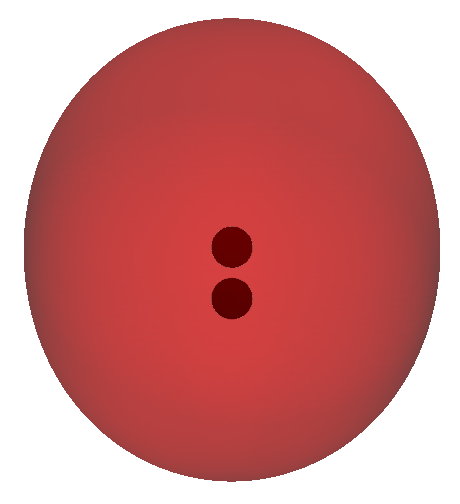
\includegraphics[width=\textwidth]{figures/h2_homo.png}
        \caption{\ce{H2} HOMO}
    \end{subfigure}
    \hfill
    \begin{subfigure}[b]{0.45\textwidth}
        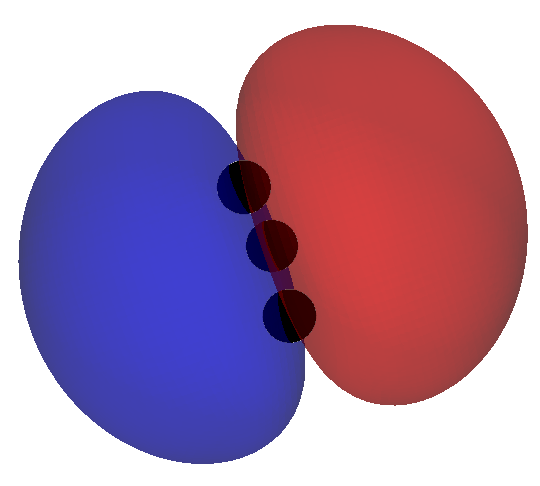
\includegraphics[width=\textwidth]{figures/h2o_homo.png}
        \caption{\ce{H2O} HOMO}
    \end{subfigure}

    \vspace{1em}

    \begin{subfigure}[b]{0.45\textwidth}
        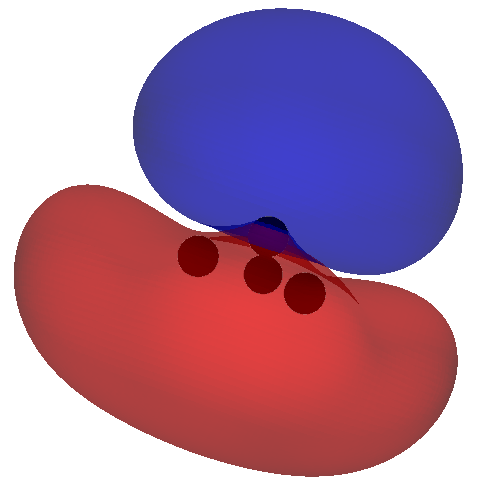
\includegraphics[width=\textwidth]{figures/nh3_homo.png}
        \caption{\ce{NH3} HOMO}
    \end{subfigure}
    \hfill
    \begin{subfigure}[b]{0.45\textwidth}
        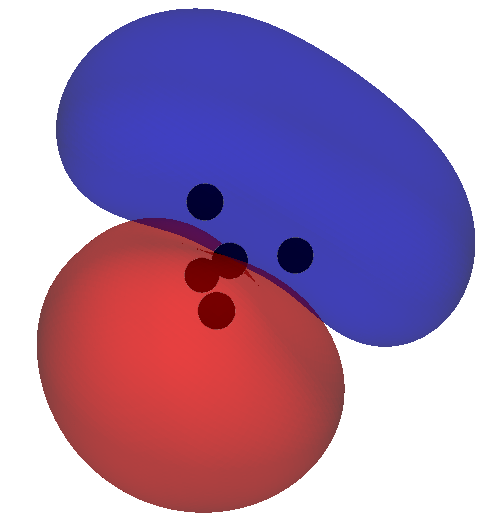
\includegraphics[width=\textwidth]{figures/ch4_homo.png}
        \caption{\ce{CH4} HOMO}
    \end{subfigure}

    \caption{3D visualizations of the HOMOs for each test molecule using isosurface rendering. Blue and red regions represent positive and negative orbital lobes, respectively.}
\end{figure}

\section{Conclusion}

This project presents a compact and functional implementation of Hartree-Fock and MP2 methods from first principles, capable of computing electronic energies and visualizing molecular orbitals for small molecules using the STO-3G basis set. The results show good agreement with reference calculations from PySCF, validating the correctness of the self-consistent field iteration, integral evaluation, and MP2 correlation energy computation.

Despite its correctness and clarity, the current implementation has several limitations. It supports only closed-shell, spin-restricted molecules, relies on a minimal basis set, and uses a memory-intensive four-index transformation for MP2 that limits scalability to larger systems. Future improvements could include open-shell and unrestricted Hartree-Fock support, larger and more flexible basis sets, and density fitting techniques to reduce the cost of MP2. Additionally, implementing more advanced correlation methods such as CCSD(T) or DFT would enhance the accuracy and applicability of the code.

\section*{References}
CCCBD Reference Values: https://cccbdb.nist.gov/energy1x.asp
\end{document}